% autoref
\documentclass[twoside,12pt]{article}
\usepackage[utf8]{inputenc}
\usepackage[russian]{babel}
\usepackage{epsfig}
\usepackage{hhline}
\usepackage{amsmath,amsfonts}
\usepackage{graphicx}
\usepackage{amssymb}
\usepackage{amsxtra}
\usepackage{amsthm}
\usepackage[mathscr]{eucal}
\usepackage{tabularx}
\usepackage{indentfirst}
\usepackage{mathtext}
\usepackage{longtable}
\usepackage{algorithmic}
\usepackage{algorithm2e}
%\usepackage[hypertex=true]{hyperref}

\pagestyle{myheadings} \tolerance=750 \setlength{\topmargin}{-0.5cm} \setlength{\headheight}{1.0cm}
\setlength{\headsep}{0.7cm} \setlength{\textheight}{23.5cm} \setlength{\oddsidemargin}{0.2cm}
\setlength{\evensidemargin}{0.2cm} \setlength{\textwidth}{15.5cm}

\def\No{$\cal N\!\!\!\raisebox{0.2ex}{\scriptsize\b{$\circ$}}$}

% Эта команда необходима для работы с установкой TeX ИТА
% Оставить эту строку закомментированной, если используется установка ИПА
%\Russian

\begin{document}

\renewcommand{\refname}{\begin{center}{\normalsize\rm \bf СПИСОК РАБОТ ПО ТЕМЕ ДИССЕРТАЦИИ }\end{center}}
\newtheorem{theorem} {Теорема}
\newtheorem{lemma} {Лемма}
\newtheorem{conseq} {Следствие}
\newtheorem{note} {Замечание}



\thispagestyle{empty}
\begin{center}
{\bf


\vskip 4em
\begin{flushright}
На правах рукописи
\end{flushright}

\vfill
{\large\bf МИРОНЕНКО Мария Андреевна}

\vskip 2em
% Если название состоит из нескольких строк, для выравнивания интервалов
% между строками \strut нужно вставлять в каждую из них
{\Large\bf
 \strut Обратные задачи в математическом моделировании помеховой обстановки на основе скрытых полумарковских моделей}

\vskip 4em
05.13.18 - Математическое моделирование, численные методы и комплексы программ

\vfill
АВТОРЕФЕРАТ

диссертации на соискание ученой степени

\mbox{кандидата физико-математических наук}

\vfill
Ростов-на-Дону\\ 2019
}
\end{center}

\eject
%---------------------------------------------------------------------------

\thispagestyle{empty}

\noindent Работа выполнена на кафедре алгебры и дискретной математики института математики, механики и компьютерных наук имени И.И.Воровича Южного федерального университета.
\vskip 2em
\noindent\underline{НАУЧНЫЙ РУКОВОДИТЕЛЬ: }

\vskip 0.5em
%
% Эту строку не трогайте.

\noindent кандидат физико-математических наук,
доцент  Деундяк Владимир Михайлович

\vskip 2em
\noindent \underline{ОФИЦИАЛЬНЫЕ ОППОНЕНТЫ:}


%
% Эту строку не трогайте.
\noindent доктор физико-математических наук,  профессор \=  \kill
%
\vskip 2em
% Если оппонентов трое, cкопируйте первую строку, а не вторую!
\noindent кандидат технических наук,
доцент

\vskip 1em
\noindent\underline{ВЕДУЩАЯ ОРГАНИЗАЦИЯ:}
\vskip 0.5em
\noindent

\vfill
% В этом абзаце можно непосредственно вставить реальные дату и время.
\noindent Защита состоится
``\underline{\hspace{2em}}''\underline{\hspace{8em}}
200\underline{\hspace{1em}}~г.
в \underline{\hspace{2em}} час. \underline{\hspace{2em}} мин.
на заседании диссертационного совета Д 212.208.25 Южного федерального университета по адресу: 347928, Ростовская область, г. Таганрог, ул. Чехова 2, ауд.\_.

\vskip 1em
Отзывы на автореферат просьба направлять по адресу:
347928, Ростовская область, г. Таганрог, пер. Некрасовский 44,
Технологический институт Южного федерального университета в г. Таганроге,
Ученому секретарю диссертационного совета Д 212.208.25 Брюхомицкому Ю.А.

\vskip 1em
\noindent С диссертацией можно ознакомиться в Зональной научной библиотеке ЮФУ по адресу: 344007, Ростовская область, г. Ростов-на-Дону, ул. Пушкинская, 148.

\vfill
% В этом абзаце можно непосредственно вставить месяц и год
\noindent Автореферат разослан
\ ``\underline{\hspace{2em}}''\underline{\hspace{8em}}
200\underline{\hspace{1em}}~г.

\vfill
\noindent Ученый секретарь \\
\noindent диссертационного совета Д 212.208.25, \\
\noindent к.т.н. \hfill Брюхомицкий Ю.А.

\eject

%---
------------------------------------------------------------------------

\setcounter{page}{1}

\centerline{\large\bf\underline{ОБЩАЯ ХАРАКТЕРИСТИКА РАБОТЫ}}
\bigskip

\textbf{Актуальность темы исследования.}
%
%
%- надо защищать информацию от помех (очень коротко, без имен)
%
%- теория кодирования, с известными фамилиями
%
%- подбор кодека, в частности ИС ОПСАПК - возможно, упомянуть области, отрасли, предприятия, где это вынуждены делать
%
%- нужны модели ошибок, их много, кто занимался, нужны общие модели
%
%- ... полиномиальное представление - возможна аппаратная реализация
%
%- обратные задачи, подбор модели к каналу; обратные задачи решать трудно, но ... смм
%
%- есть смм, моделирует системы с состояниями... умеют решать, в частности, обратные задачи...

Для обеспечения высококачественной передачи информации в последние десятилетия широко используются цифровые системы передачи данных. Цифровая передача данных предоставляет больше возможностей в обработке информации по сравнению с аналоговой, цифровые каналы менее подвержены искажению и интерференции, а применение процедур обнаружения и исправления ошибок делают возможной высокую точность сигнала. Для обнаружения и исправления ошибок эффективно используются средства алгебраического помехоустойчивого кодирования. За последние полвека было разработано большое количество алгебраических кодов, исправляющих ошибки, в частности,  коды Хэмминга, Боуза-Чоудхури-Хоквингема, Рида-Соломона, Рида-Маллера, циклические, сверточные и др. В настоящее время продолжается разработка новых кодов и алгоритмов декодирования. Важные результаты в этой области получены М. Суданом, В.М. Сидельниковым, С.А. Осмоловским и ... (еще три строчки фамилий, может быть с конкретизацией областей или (и) стран, городов, институтов) другими учеными.

При применении помехоустойчивого кодирования следует учитывать, что различные коды и алгоритмы их декодирования неодинаково хорошо справляются с разными типами ошибок. Поэтому нужно уметь подбирать для каждого конкретного канала наиболее эффективные методы и средства обнаружения и исправления ошибок. Для решения этой задачи необходимо иметь достаточный объем сведений о возможных помехах в канале и о корректирующих свойствах кода по отношению к ошибкам различной структуры. Подбор помехоустйчивого кодека к реальному каналу является сложной задачей оптимизации соотношения между затратами на кодирование и обеспечиваемым качеством передачи информации. Проведение реальных экспериментов, как правило, достаточно трудоемко, поэтому эффективным оказывается применение имитационного моделирования помехоустойчивых каналов связи. Основанные на имитационном моделировании системы оценки применимости схем алгебраического помехоустойчивого кодирования позволяют подбирать помехоустойчивые кодеки по потокам ошибок, порождаемым математическими моделями источников ошибок. Схема информационной системы оценки применимости схем алгебраического помехоустойчивого кодирования была построена в работах Н.С. Могилевской. Предложенная система позволяет решать такие задачи как согласование помехоустойчивого кодека с каналом, изучение корректирущих свойств декодеров, исследование быстродействия работы кодера и декодера и многие другие.

Важную роль в работе предложенной информационной системы играют модели источников потоков ошибок, имитирующие внешние воздействия в канале связи. Моделированием источников потоков ошибок занимались такие ученые как Э.Н. Гильберт, Е.О. Эллиот, Б.М. Игельник, В.И. Петрович, Б.Д. Фричман, В.М. Охорзин, В.О. Колпаков, В.Я. Турин, О.В. Попов, Ю.С. Чье и другие. В настоящее время известно множество классических моделей источников ошибок, однако, как правило математическая модель источника ошибок описывает узкий класс каналов связи, поэтому для исследования корректирующей способности кодека по отношению к различным типам ошибок при проведении имитационных экспериментов необходимо использовать несколько моделей источников ошибок. Это затрудняет проведение имитационных экспериментов, поскольку в их процессе приходится тестировать корректирующую способность кодеков для разных моделей. Представляется более удобным построить общую модель источника ошибок канала, которая учитывала бы $q$-ичные алфавиты и позволила бы моделировать различные случаи помеховой обстановки путем изменения параметров.

Для проведения имитационных экспериментов, направленных на подбор кодека к конкретному каналу связи, важно, чтобы используемая модель канала связи соответствовала реальному каналу связи, для которого подбирается кодек. Поэтому необходимо научиться решать задачу адекватного представления зарегистрированной в реальном канале последовательности ошибок математической моделью источника ошибок, чтобы впоследствии использовать эту модель в качестве генератора потоков ошибок при проведении имитационных экспериментов с целью подбора кодека.

Таким образом, актуальным представляется построение общей математической модели источника ошибок в канале передачи данных и разработка алгоритма подбора адекватной модели источника ошибок для конкретного канала связи.

\textbf{Целью диссертационной работы} является построение общей математической модели источника ошибок в канале передачи данных, разработка алгоритмов, численных методов и программного комплекса, позволяющих осуществлять генерацию потоков ошибок в соответствие с построенной моделью и подбор адекватной математической модели источника ошибок для конкретного канала связи.

\textbf{Задачами диссертационной работы} являются:
 \begin{enumerate}
   \item {Провести содержательный анализ и систематизацию сведений о существующих способах моделирования источников потоков ошибок и определить математический аппарат, позволяющий построить такую общую математическую модель источника ошибок, для которой возможно решение задачи подбора конкретной модели, соответствующей зарегистрированной в канале передачи данных последовательности ошибок.}
   \item {Разработать общую модель источника ошибок на основе теории скрытых марковских и полумарковских моделей.}
   \item {Разработать численные методы, позволяющие для реального канала передачи данных подбирать адекватную математическую модель источника ошибок.}
   \item {Усовершенствовать информационную систему оценки применимости схем алгебраического помехоустойчивого кодирования, расширив ее функционал возможностью подбирать подходящую модель источника ошибок для исследуемого реального канала связи.}
   \item {Разработать программный комплекс для исследования моделей источников ошибок, позволяющий как генерировать потоки ошибок с помощью разработанных ранее моделей, так и подбирать наилучшую модель по реальному потоку ошибок в канале.}
 \end{enumerate}
 \textbf{Методология и методы исследования.} При выполнении работы использовались методы алгебры, теории конечных автоматов, теории вероятностей, математической статистики, компьютерного эксперимента. Существенно применялась теория скрытых марковских и полумарковских моделей, в частности, методы решения задач оценивания. Для реализации вычислительного ядра программного комплекса использовался язык программирования $C\sharp$, пользовательский интерфейс реализован посредством интерфейса программирования приложений Windows Forms. При разработке архитектуры программного комплекса и в ходе программной реализации соблюдались принципы объектно-ориентированного проектирования, исходный код программного комплекса покрыт модульными и интеграционными тестами.

\textbf{Достоверность научных результатов} подтверждается точностью постановок задач, совпадением частных случаев предлагаемых моделей с классическими моделями, обоснованностью принятых предположений и допущений, приведенным доказательством новых и корректным применением известных теоретических положений, корректным применением методов и алгоритмов, устойчивой работой разработанного программного комплекса и результатами численных экспериментов, проведенных на модельных примерах.

 \textbf{Объектом исследования диссертационной работы} являются потоки ошибок в цифровых помехоустойчивых каналах связи.

 \textbf{Предметом исследования} выступают методы моделирования и анализа потоков ошибок в цифровых каналах передачи данных.

 \textbf{Тематика работы} соответствует п.1 «Разработка новых математических методов моделирования объектов и явлений.», п.3 «Разработка,  обоснование  и  тестирование  эффективных  вычислительных методов с применением современных компьютерных технологий»,п.4 «Реализация  эффективных  численных  методов  и  алгоритмов  в  виде комплексов  проблемно-ориентированных  программ  для  проведения вычислительного эксперимента» и п.8 «Разработка систем компьютерного и имитационного моделирования» паспорта специальности 05.13.18 – «Математическое моделирование, численные методы и комплексы программ».

\textbf{Научная новизна.} В диссертации получены следующие новые научные и практические результаты:
\begin{itemize}
  \item {\textit{в области математического моделирования:}
\begin{itemize}
  \item {разработаны три новых модели источника ошибок в $q$-ичном цифровом канале передачи данных --- скрытая марковская модель источника ошибок, скрытая полумарковская модель Фергюсона и скрытая полумарковская $QP$-модель, позволяющие имитировать различные случаи помеховой обстановки, совпадающие в частных случаях со многими широко применяющимися моделями источников ошибок и отличающиеся от существующих возможностью решения для них задачи подбора модели с такими параметрами, что она сможет адекватно имитировать конкретный реальный канал связи. Все предложенные модели позволяют моделировать потоки ошибок в $q$-ичном цифровом канале с несколькими физическими состояниями. Скрытая марковская модель источника ошибок является обобщением классических моделей Гильберта и Фричмана и предполагает, что длительность пребывания в состоянии описывается геометрическим распределением. Отличие скрытой полумарковской модели Фергюсона заключается в явном задании длительности пребывания модели в состоянии, при этом распределение вероятностей ошибок внутри состояния является равномерным. Наиболее важной с точки зрения научной новизны является скрытая полумарковская $QP$-модель, позволяющая как и модель Фергюсона явно моделировать длительность пребывания в состоянии, а также задавать произвольное распределение вероятностей ошибок на протяжении состояния.}
  \item {построена модификация модели информационной системы оценки применимости схем помехоустойчивого алгебраического кодирования, в рамках которой впервые предложено использование скрытых полумарковских моделей в качестве базовых моделей источника ошибок и добавлен новый модуль подбора адекватной реальному каналу модели источника ошибок (из базы данных моделей источников ошибок информационной системы). Такая модификация позволяет решить в рамках информационной системы оценки применимости схем помехоустойчивого алгебраического кодирования ранее не ставившийся вопрос адекватности имитационной модели канала реальному каналу связи}.
\end{itemize}
  }
  \item {\textit{в области численных методов:}
  \begin{itemize}
  \item {впервые предложен и теоретически обоснован алгоритм подбора по зарегистрированной в реальном канале передачи данных последовательности ошибок адекватной математической модели источника ошибок из заранее определенного набора моделей. Этот алгоритм опирается на разработанный и теоретически обоснованный в работе алгоритм вычисления вероятности, с которой модель источника ошибок смогла бы сгенерировать рассматриваемую последовательность ошибок, и представляет собой модификацию для случаев скрытой полумарковской модели Фергюсона и скрытой полумарковской $QP$-модели алгоритма прямого хода, описанного в работах Шенг Женг Ю.}
\end{itemize}
}
  \item {\textit{в области комплексов программ:}
  \begin{itemize}
  \item {разработан и протестирован новый программный комплекс, направленный на исследование моделей источников ошибок и позволяющий решать такие задачи как генерация последовательности ошибок моделью с заданными параметрами, вычисление вероятности генерации некоторой заданной последовательности исследуемой моделью, подбор по имеющейся последовательности ошибок наиболее адекватной модели из некоторого набора.
       %Комплекс поддерживает скрытую марковскую модель, скрытую полумарковскую модель Фергюсона и скрытую полумарковскую $QP$-модель, несколько типов генераторов случайных чисел, несколько критериев адекватности модели последовательности ошибок.
       }
      %Архитетура комплекса?%
\end{itemize}
}
\end{itemize}


\textbf{Основные положения}, выносимые на защиту.
\begin{itemize}
  \item Скрытая полумарковская $QP$-модель источника ошибок в $q$-ичном цифровом канале передачи данных, которая обобщает ряд классических моделей источников ошибок и которую в силу общности и особенностей структуры целесообразно впоследствие включить в ИС ОПСАПК.
  \item Полиномиальное представление скрытой полумарковской модели фергюссоновского типа, ускоряющее процесс генерации последовательностей ошибок, а также алгоритм его построения.
  \item Алгоритм численного решения задачи оценивания для общей скрытой полумарковской модели, его полное теоретическое обоснование и адаптация на случай скрытой полумарковской $QP$-модели и скрытой полумарковской модели фергюсоновского типа.
  \item Схема подбора модели источника ошибок из базы скрытых полумарковских моделей по реальной канальной последовательности и модификация информационной системы оценки применимости схем помехоустойчивого кодирования (ИС ОПСАПК) на ее основе.
  \item Программный комплекс, позволяющий генерировать потоки ошибок и подбирать наиболее адекватную модель источника ошибок по канальной последовательности ошибок.
%
\end{itemize}

%\textbf{Научная новизна работы}. Построена новая универсальная модель источника ошибок в цифровом канале (скрытая полумарковская QP-модель), позволяющая моделировать различные типы помеховой обстановки, в частности группирование ошибок в пакеты, и включающая в себя как частные случаи многие классические модели источников ошибок. Предложено использование в качестве модели источника ошибок скрытой полумарковской модели Фергюсоновского типа и для этой модели разработан алгоритм построения полиномиальной схемы, позволяющий значительно ускорить процесс генерации последовательностей ошибок. Для обеих моделей источников ошибок разработан алгоритм подбора по зарегистрированной в реальном канале последовательности ошибок модели источника ошибок из некоторого конечного набора моделей того же типа. Для этого были решены задачи оценивания для обоих типов моделей.
%Предложена модификация информационной системы оценки применимости схем помехоустойчивого кодирования (ИС ОПСАПК),в рамках которой предложено использование в качестве базовых моделей источника ошибок скрытых полумарковских моделей и добавлен модуль подбора модели источника ошибок, адекватной конкретному каналу связи.

\textbf{Теоретическая ценность} диссертационной работы состоит в разработке новых математических моделей источника ошибок в $q$-ичных цифровых каналах передачи данных, постановке и решении задачи адекватного представления помеховой обстановки в канале передачи данных математической моделью источника ошибок, построении и теоретическом обосновании алгоритмов подбора математической модели источника ошибок по зарегистрированной в канале последовательности ошибок, разработке алгоритма построения полиномиального представления скрытой полумарковской модели фергюсоновского типа.

\textbf{Практическая ценность} диссертационной работы заключается в построении модификации информационной системы оценки применимости схем помехоустойчивого кодирования, позволяющей решать нерешенную ранее задачу подбора адекватной математической модели источника для описания помеховой обстановке в исследуемом канале; разработке программного комплекса, позволяющего генерировать потоки ошибок с помощью новых моделей источников ошибок, а также реализующего несколько вариантов алгоритма подбора наиболее соответствующей модели источника ошибок по последовательности ошибок.

%\textbf{Теоретическая ценность}
%1. модель, полиномиальное....
%
%2. алгоритмы...
%
%\textbf{Практическая ценность}... полученные результаты... и разработаный программный комплекс позволяют модифицировать реализацию инф систему...

\textbf{Реализация результатов работы. }

\textbf{Апробация диссертационной работы.}
Основные результаты работы докладывались~на XI Всероссийском симпозиуме по прикладной и промышленной математике (весенняя сессия,г. Кисловодск, 1 - 8 мая 2010 г.), на международной научно-практической конференции "Информационная безопасность 2010". (г. Таганрог, 22-25 июня 2010г.), XVIII Всероссийской Школе-Коллоквиуме по стохастическим методам (весенняя сессия, Казань, 1 - 8 мая 2011 г.), на международной научно-практической конференции "Современные проблемы и достижения в отраслях радиотехники, телекоммуникаций и информационных технологий". (Украина, г. Запорожье, 19 - 21 сентября 2012 г), на V международной конференции "Современные методы и проблемы теории операторов и гармонического анализа и их приложения" (г. Ростов-на-Дону, 26 апреля-1 мая 2015 г.),на 4-й Российско-Китайской конференции Numerical Algebra with Applications (г. Ростов-на-Дону, 26-29 июня 2015 г.), на Международной конференции молодых ученых стран БРИКС (г. Ростов-на-Дону, 24-26 сентября 2015 г.), на VI Международной конференции "Современные методы и проблемы теории операторов и гармонического анализа и их приложения" (г. Ростов-на-Дону, 24 апреля-29 апреля 2016 г.).

\textbf{Публикации.} Основные результаты по теме диссертации изложены в 16 печатных изданиях ~\cite{BibZhd_2009}--\cite{DeMoZhd_DSTU}, четыре из которых изданы в журналах, рекомендованных ВАК для публикации научных работ, отражающих основное содержание диссертации ~\cite{DeZhda_VGU13}, \cite{DeZhd_DSTU14}, \cite{DeZhda_Izvestia2015}, \cite{DeMoZhd_DSTU}, четыре --- в журналах и сборниках научных работ,
девять --- в тезисах международных и всероссийских научных конференций. В работах \cite{DeZhda_Ivan}, \cite{DeZhda_Obozr11}, \cite{DeZhda_Obozr10}, \cite{DeZhda_VGU13}, \cite{DeZhd_DSTU14} научному руководителю В.М. Деундяку принадлежат обсуждения формулировки результатов и методов их получения, в работах \cite{BibZhd_2009}, \cite{BibZhd_2010} автору диссертации принадлежит разработка математической и компьютерной модели источника ошибок; в работах \cite{DeMoZhd_Sim}, \cite{DeMoZhd_conf16}, \cite{DeMoZhd_DSTU} автору диссертации принадлежит разработка метода подбора адекватной модели потока ошибок к реальному каналу связи и модификация ИС ОПСАПК на основе автоматизированного выбора модели источника ошибок.

\textbf{Структура работы и объем диссертации.}
Работа состоит из введения, четырех глав, заключения и библиографического списка.

\textbf{Во введении} дается общая характеристика работы и приводятся основные результаты диссертационной работы.

\textbf{Первая глава} посвещена обзору методов и проблем математического моделирования цифровых помехоустойчивых каналов связи. Логически она подразделяется на два раздела. В первом разделе приведены сведения о цифровых помехоустойчивых каналах связи, имитационном моделировании таких каналов, моделях источников ошибок и задачах, возникающих при имитационном моделировании. Во втором разделе изложены основы математического аппарата теории скрытых марковских и полумарковских моделей, необходимые для дальнейшего изложения. В итоге формулируется как актуальная задача подбора математической модели помех для описания реальной помеховой обстановки.

%В последние десятилетия цифровые системы передачи данных становятся все более и более востребованными. Цифровая передача данных предоставляет больше возможностей в обработке информации по сравнению с аналоговой, цифровые каналы менее подвержены искажению и интерференции, а применение процедур обнаружения и исправления ошибок делают возможной высокую точность сигнала.
%
%Основную задачу теории и техники связи составляет передача сообщений из одного пункта в другой. Под \textit{системой передачи информации} или \textit{системой связи} понимают совокупность передатчиков, приемников и каналов, обеспечивающих обмен сообщениями между пунктами связи. \textit{Каналом} связи называют совокупность средств передачи информации, включающую в себя физическую среду. Для любой физической среды, используемой для передачи информации, существенно, что передаваемый сигнал подвержен случайным искажениям.
...В работе рассматриваются $q$-ичные идеально синхронизированные, симметричные, нестационарные каналы с памятью.

... возникают помехи, используются кодеки, 
%Цифровой канал называется $q$-ичным, если его алфавит имеет мощность $q$. В случае, когда мощность алфавита --- степень простого числа, в качестве алфавита, как правило, рассматривается поле Галуа $F_q$. $q$-ичный канал называется \textit{симметричным}, если в канале вероятность замещения символа $a$ каким-то другим символом $b$, отличным от $a$, от значения $b$ не зависит. Канал, в котором каждый символ выходной последовательности зависит не только от соответствующего символа на входе, но и от предыдущих символов, называется каналом с памятью.
%Каналы связи называют идеально \textit{синхронизированными}, если в них есть механизмы, позволяющие препятствовать влиянию ошибок типа выпадения и вставки символов. Канал связи называется \textit{стационарным}, если его статистические характеристики не зависят от времени.

% В общем случае реальные каналы связи неидеально синхронизированы, нестационарны, несимметричны и имеют память, однако учесть при моделировании канала одновременно влияние всех этих факторов достаточно сложно. Поэтому далее в работе рассматриваются идеально синхронизированные, симметричные, нестационарные каналы с памятью.

При использовании каналов связи необходимо учитывать возможность возникновения в них ошибок. В зависимости от характеристик в реальном канале передачи данных могут возникать как одиночные ошибки, так и пакеты ошибок различной структуры и длительности. Для борьбы с ошибками применяются помехоустойчивые коды, принципом работы которых является внесение кодером избыточности в информационную последовательность и последующее использование ее при декодировании для обнаружения и исправления ошибок. Следует отметить, что различные коды и алгоритмы их декодирования неодинаково хорошо справлются с различными типами ошибок. Поэтому нужно уметь подбирать для каждого конкретного канала наиболее эффективные методы и средства обнаружения и исправления ошибок.

Решение этой задачи в аналитическом виде является сложным, поэтому эффективным представляется подбор помехоустойчивого кодека на основе проведения экспериментов с использованием имитационных моделей каналов с помехами и анализа их результатов. Эта задача может быть решена в рамках информационной системы оценки применимости схем алгебраического помехоустойчивого кодирования (ИС ОПСАПК).

%Под информационной системой оценки применимости схем алгебраического помехоустойчивого кодирования будем понимать систему, позволяющую на основе компьютерных имитационных экспериментов оценить корректирующие способности помехоустойчивых алгебраических кодеков по отношению к ошибкам различного типа и подобрать оптимальный по заданным параметрам кодек к конкретному каналу связи.
%
%В основе системы лежит имитационная модель цифрового помехоустойчивого канала, рассмотренная в предыдущем разделе. Также в состав входят база данных БД, содержащая информацию об условиях и результатах проведенных имитационных экспериментов, и блок анализа записей базы данных БАЗ, который осуществляет работу с данными БД.

Для функционирования информационной системы типа ИС ОПСАПК, описанной в предыдущем разделе, необходимо научиться решать задачу адекватного представления зарегистрированной в реальном канале последовательности ошибок математической моделью источника ошибок, чтобы впоследствии использовать эту модель в качестве генератора потоков ошибок при проведении имитационных экспериментов с целью подбора кодека. В силу того, что ИС ОПСАПК хранит результаты ранее проведенных экспериментов, интерес представляет не столько построение новой, адекватной каналу в смысле некоторого критерия модели источника ошибок, сколько подбор наилучшей модели из уже имеющихся в библиотеке моделей источников ошибок.

Далее будем говорить о задаче подбора модели источника ошибок как об \emph{обратной задаче}, понимая под \emph{прямой} задачу генерации моделью последовательности ошибок.

%Разработкой моделей источников ошибок занимались многие ученые: Э.Н. Гильберт, Е.О. Эллиот, Б.М. Игельник, В.И. Петрович, Б.Д. Фричман, В.М. Охорзин, В.О. Колпаков, В.Я. Турин, О.В. Попов, Ю.С. Чье и другие.
%Выделяют несколько подходов к математическому моделированию источников ошибок: на основе цепей Маркова, на основе процессов восстановления, на основе процессов накопления,а также на основе теории квазипериодических последовательностей случайных величин. Как правило, математическая модель описывает некоторый узкий класс каналов, поэтому для исследования корректирующей способности кодека по отношению к различным типам ошибок при проведении имитационных экспериментов необходимо использовать несколько моделей источников ошибок.

Представляет интерес построение моделей источника ошибок на основе скрытых полумарковских моделей, поскольку модели позволяют моделировать системы с несколькими состояниями и способны порождать последовательности наблюдений различной структуры. Кроме того, перспективным представляется использование методов статистического анализа, разработанных для скрытых полумарковских моделей, для подбора модели источника ошибок к каналу связи.

\textbf{Вторая глава} посвящена построению моделей источников ошибок в $q$-ичных цифровых каналах связи на основе скрытых марковских и полумарковских моделей. В частности, в главе строятся скрытая марковская модель источника ошибок, скрытая полумарковская $QP$-модель источника ошибок и скрытая полумарковская модель источника ошибок Фергюсоновского типа. Для модели Фергюсоновского типа строится полиномиальное представление. В заключительной части главы описывается программный комплекс HsmmErrorSourceGeneration, предназначенный для генерации последовательностей ошибок на основе построенных ранее в главе моделей источников ошибок.

Под \textbf{скрытой полумарковской QP-моделью} (CПМQP-моделью) источника ошибок будем понимать набор $$\lambda =  \{\mathcal{S};\mathcal{D}; A; \Pi; p(d); \rho; \mu ;M ;{\mathbb{F}}_q;B \},$$
параметры которого определяются следующим образом.

1) $\mathcal{S}=\{1,...,N\}$ --- алфавит состояний дискретной полумарковской цепи, $\mathcal{D}=\{1,...,D\}$ -- алфавит возможных длительностей состояний.

2) $A=\{a_{ii^\prime}\}_{i,i^\prime\in \mathcal{S}}$ --- матрица переходных вероятностей, матричный элемент $a_{ii^\prime}$ которой представляют собой вероятность перехода из состояния $i$ в состояние $i^\prime$, то есть
$$\forall i,i^\prime \in \mathcal{S}: \;\;\; a_{ii^\prime} \triangleq P_\nu[S_{[t}=i^\prime|S_{t-1]}=i],$$
где $t$ --- момент времени, когда произошёл переход из обобщённого состояния $(i,d)$ в $(i^\prime,d^\prime)$. Для матрицы $A$ должно также выполняться условие стохастичности, то есть:
$$\forall i,i^\prime \in \mathcal{S}: 0\leq a_{ii^\prime} \leq 1$$
и
$$\forall i \in \mathcal{S}: \sum\limits_{i^\prime\in \mathcal{S}} a_{ii^\prime}=1.$$

3) $\Pi=\{\pi_{i}\}_{i\in \mathcal{S}}$ представляет собой исходное распределение вероятностей состояний. Элемент $\pi_{i}$  --- вероятность того, что система прибывала в состоянии $i$ до начала наблюдений. Таким образом, можно записать:
$$\forall i\in \mathcal{S}:\;\;\; \pi_{i}\triangleq P[S_{0}=i].$$

4) $p(d)=\{p_i(d)\}_{i\in\mathcal{S}}$ --- набор распределений вероятностей длительностей в различных состояниях, где $p_i(d)$ соответствует вероятности наблюдения состояния $i$ на протяжении в точности $d$ моментов времени. Сказанное можно записать в виде:
$$\forall (i,d) \in \mathcal{S}\times \mathcal{D}: \;\;\; p_i(d)\triangleq P[S_{t+1:t+d]}=i|S_{[t+1}=i].$$

5) $\rho=\{\rho_i(l)\}_{i\in\mathcal{S}, l \in L_i}$ --- вектор, составленный из эталонных плотностей, определяемых на эталонных отрезках $L=\{L_i\}_{i\in\mathcal{S}}$ длин $\Delta=\{\delta_i\}_{i\in\mathcal{S}}$, где
$$\forall i\in \mathcal{S}, l \in L_i :\;\;\; 0\leq \rho_i (l)\leq 1$$
и
$$\forall i\in \mathcal{S}:\;\;\; \sum\limits_{l\in L_i} \rho_i(l)=1.$$
$\mu=\{{\mu}_i\}_{i\in\mathcal{S}}$ --- вектор средних вероятностей появления ошибки в различных состояниях, a $M$ --- средняя вероятность появления ошибки в канале. Для эталонных плотностей $\rho_i$ должно также выполняться условие адаптированности к каналу:
$$\forall i\in \mathcal{S}, \forall l \in L_i :\;\;\; \rho_i(l)\leq \frac{1}{\delta_i \mu_i}\leq 1.$$

6) Поле Галуа $F_q$ --- алфавит наблюдаемых символов. $\mathbb{F}^\ast_q$ --- мультипликативная группа поля Галуа $\mathbb{F}_q$. $B=\{b_{i}(k)\}_{i \in \mathcal{S}, k \in \mathbb{F}^\ast_q}$ --- набор распределений вероятностей значений ошибки в состояниях, элемент которого $b_{i}(k)$ представляет собой вероятность наблюдать символ $k$ в состоянии $i$, т.е. можно записать в виде:
$$\forall i \in \mathcal{S},\forall k \in \mathbb{F}^\ast_q :$$
$$\;\;\; b_{i}(k)\triangleq P[k|S_{t}=i].$$

Посредством описанной модели можно производить генерацию потоков ошибок. В нулевой момент времени (то есть до начала генерации последовательности ошибок) с помощью вектора $\Pi$ определяется состояние системы до наступления первого момента времени. Далее для каждого момента времени выполняется следующая последовательность действий:

1) На основе матрицы переходных вероятностей выбирается текущее состояние канала $i$.

2) С использованием распределения вероятностей длительностей $p_i(d)$ в выбранном состоянии определяется длина $d$ временного отрезка, на протяжении которого модель будет находиться в текущем состоянии (то есть длительность текущего состояния).

3) Для каждой точки отрезка выбранной длины вычисляется вероятность наличия в ней ошибки:
\begin{equation}
\label{eq_error_prob}
\forall \theta \in [1,d]: e_{i,\theta}^d = \varphi_i^d(\theta)\mu_i d,
\end{equation}
где
\begin{equation}
\label{eq_varphi}
\varphi_i^d(\theta) = \int\limits_{\theta}^{\theta+1} \varphi_{i,d}^{pc}(x)dx
\end{equation}
и
$$\forall l\in L_i: \;\;\;\;\; \varphi_{i,d}^{pc}\mid _{(lq,(l+1)q]}=\frac{\delta_i}{d}\cdot \rho(i),$$

\noindent где $q=\frac{d}{\delta_i}$. В соответствии с этой вероятностью определяется наличие ошибки на данной позиции.

4) В случае, если ошибка есть, в соответствии с матрицей $B$ генерируется ее значение. В противном случае, на этой позиции будет стоять нулевой элемент.

\textbf{Скрытой полумарковской моделью фергюсоновского типа} будем называть систему:
\begin{equation}\label{chapt2_Ferguson_model:def} \Delta =\{S,A,\pi,V,B,D,F\},\end{equation}
где
1) $S=\{S_1,S_2,...,S_N\}$ -- алфавит состояний модели;

2) $A=\{a_{ij}\}_{i,j=1}^N$ -- матрица переходов;

3) $\pi=\{\pi_i \}_{i=1}^N$ –- вектор начального распределения вероятностей состояний;

4) $V=\{v_1,v_2,...,v_M\}$ –- алфавит наблюдаемых символов;

5) $B=\{b_{ij}\}_{i,j=1}^{N,M}$–- матрица условных вероятностей наблюдения символа $v_j$ в состоянии $S_i$;

6) $D$ –- алфавит возможных длительностей мощности $L$;

7) $F=\{f_{ij}\}_{i,d=1}^{N,L}$ –- матрица размера $N\times L$, элемент $f_{ij}$  которой представляет собой вероятность наблюдать длительность $d_j$ при условии, что $\Delta$ находится в состоянии $S_i$.

Процесс генерирования последовательности наблюдений посредством модели типа Фергюсона выглядит следующим образом.

 \textbf{Этап 1.} В соответствии либо с вектором $\pi$ (в момент времени $t=1$ ), либо с матрицей $A$ выбирается текущее состояние.

 \textbf{Этап 2.} В выбранном состоянии $S_i$ с использованием $p_i(d)$ определяется длина временного промежутка, втечение которого система будет находиться в $i$-ом состоянии.

 \textbf{Этап 3.} В каждой точке этого отрезка посредством $b_i(k)$ генерируется наблюдение.

\textbf{Полиномиальной моделью скрытой полумарковской модели типа Фергюсона} назовем систему
$$\Pi M=(u^A,u^B,u^F,f_B (x_B,f_A (x_A,q_A )),f_F (x_F,f_A (x_A,q_A )),\pi),$$
в которой $u^A$,$u^B$ и $u^F$ –- случайные величины, определяемые по разложениям матриц $A$, $B$ и $F$ на линейные комбинации простых матриц, значения которых закодированы элементами поля $F_{2^n}$.
Структурная схема автомата, реализующего полиномиальное представление скрытой полумарковской модели фергюсоновского типа $\Delta$, представлена на рисунке \ref{fig:chapt2_Ferguson:scheme}.

\begin{center}\label{fig:chapt2_Ferguson:scheme}
  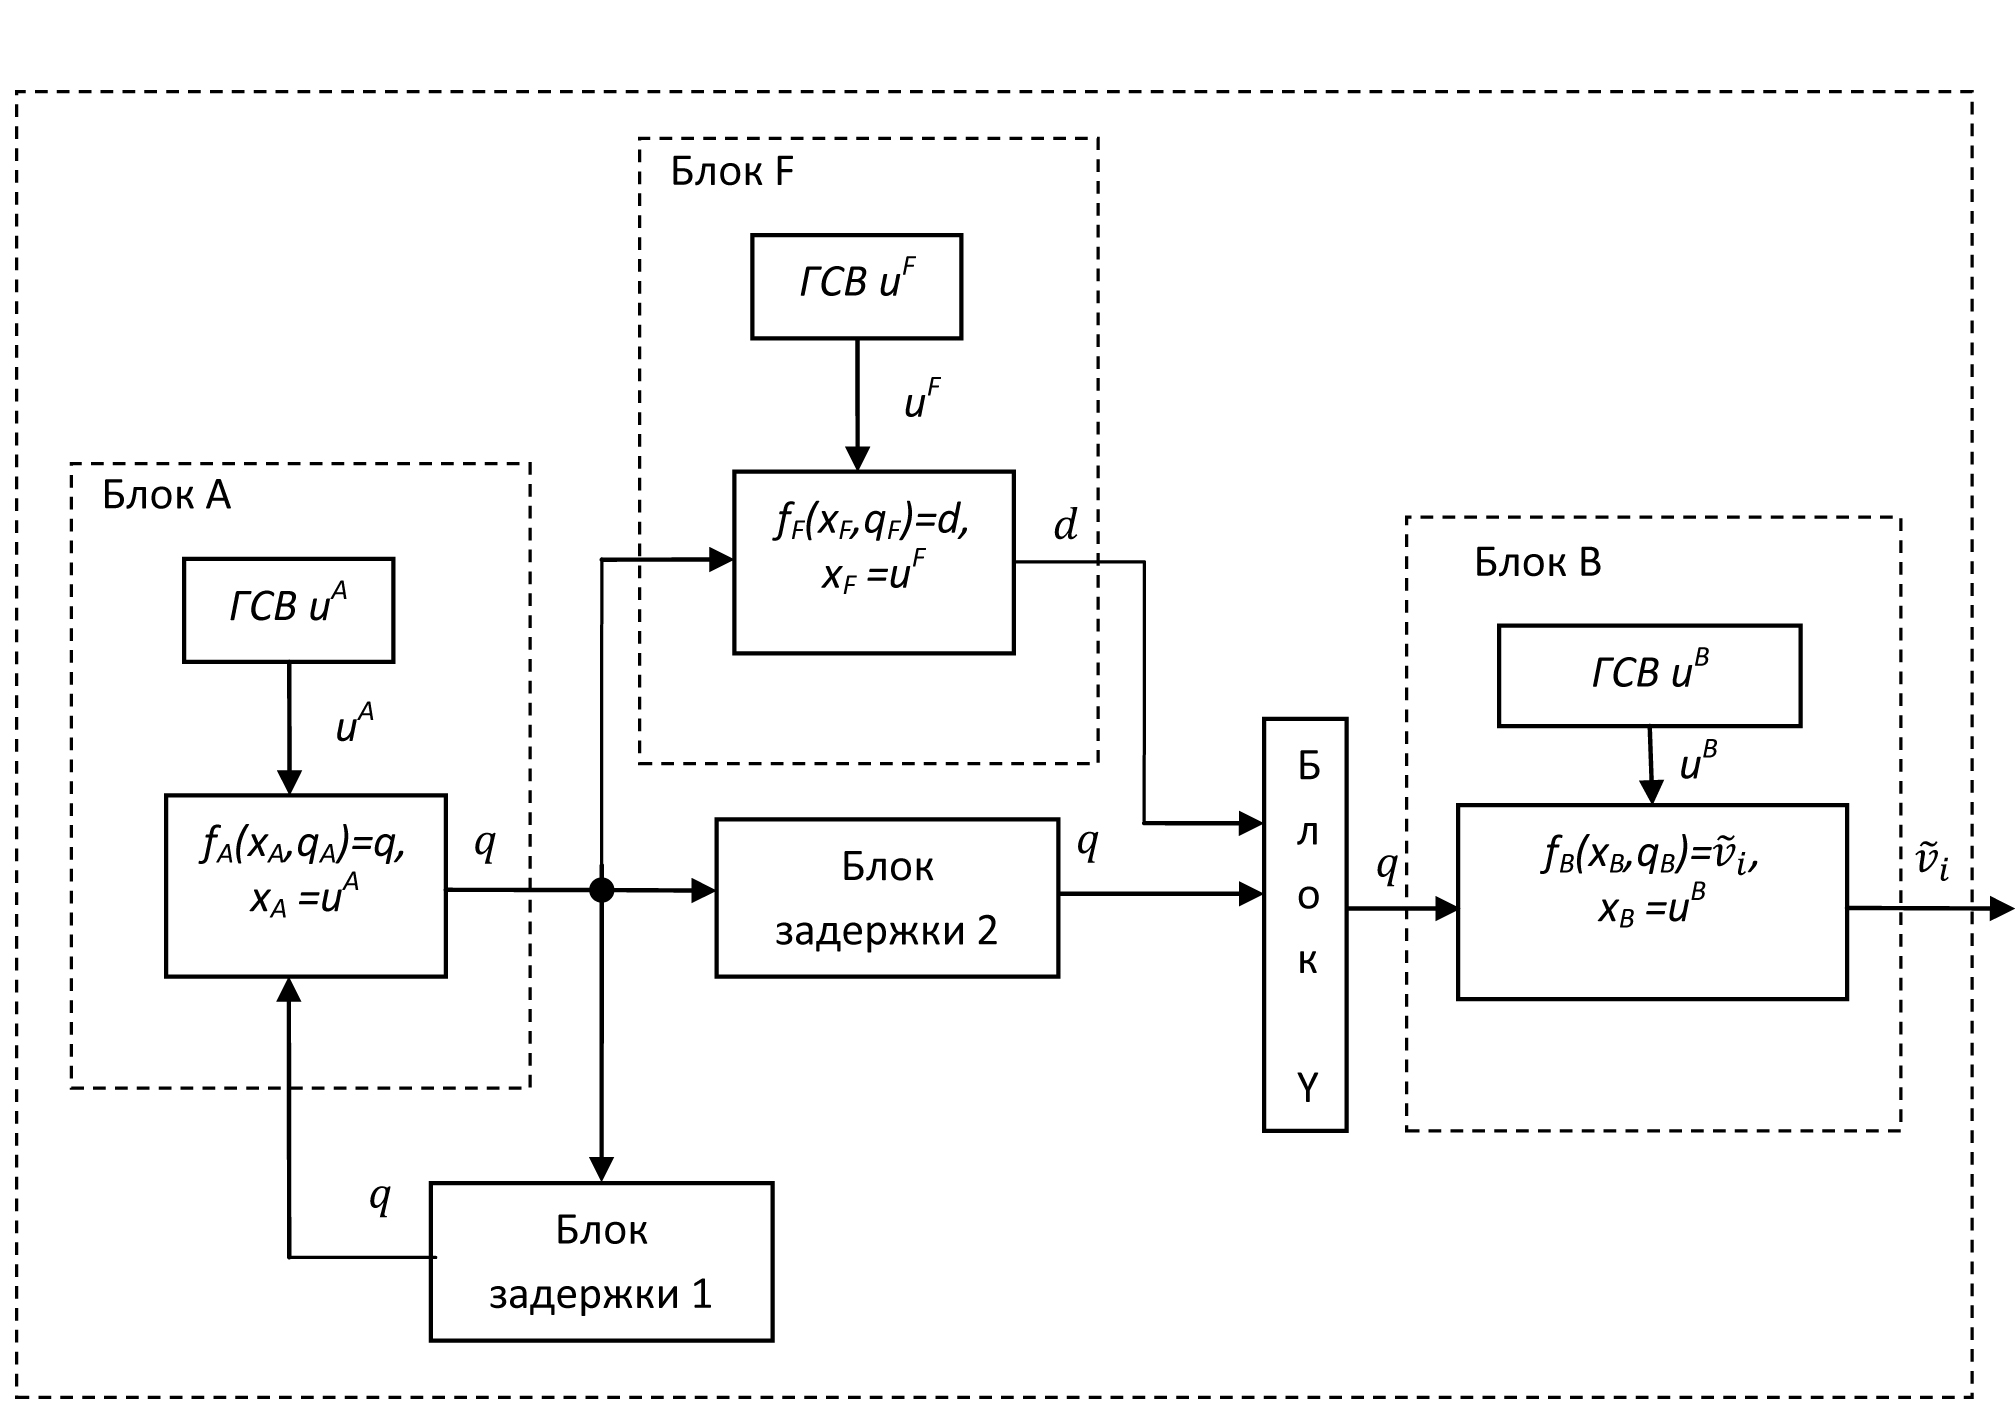
\includegraphics[height=100mm]{Structural_model.jpg}
 Рис 1. Структурная схема автомата, реализующего полиномиальное представление скрытой полумарковской модели типа Фергюсона.
  \end{center}

Для генерации потоков ошибок скрытой полумарковской $QP$-моделью и скрытой полумарковской моделью Фергюсоновского типа разработан специальный комплекс программ \textbf{HsmmErrorSourcesGeneration}. Основной задачей этого програмного комплекса является предоставление исследователю возможности осуществлять генерацию последовательностей ошибок в соответствии с заданными в виде текстового файла параметрами модели источника ошибок и алгоритмом генерации для модели заданного типа. Полученные на выходе текстовые файлы, содержащие сгенерированные последовательности, могут использоваться исследователем для самостоятельного анализа.

Программный комплекс \textbf{HsmmErrorSourcesGeneration} реализован на языке программирования высокого уровня $C\sharp$. Необходимым условием для работы программного продукта является наличие .NET Framework 4.0. В основе архитектуры комплекса лежат принципы объектно-ориентированного дизайна.

\textbf{В третьей главе} предлагаются алгоритмы решения задачи оценивания в случае общей скрытой полумарковской модели, скрытой полумарковской модели Фергюсона и скрытой полумарковской $QP$-модели, а также задачи подбора модели источника ошибок из набора моделей, позволяющей наилучшим образом генерировать заданную последовательность ошибок.

Эта задача не имеет решения в общем виде, но может быть решена для скрытых марковских и полумарковских моделей. В этом случае ее решение основывается на решении \textit{задачи оценивания}, т.е. на вычислении вероятности генерации последовательности ошибок заданной скрытой полумарковской моделью. В работе Рабинера предлагается алгоритм решения задачи оценивания для скрытых марковских моделей, а Ю предлагает ее решение для общих скрытых полумарковских моделей при дополнительных предположениях относительно начала и конца скрытой последовательности состояний, а именно, что первое наблюдаемое состояние началось в или до первого наблюдаемого момента времени, а последнее состояние закончилось строго в момент времени $T$.

В главе рассматриваются и теоретически обосновываются два варианта решения задачи оценивания для случая общей скрытой полумарковской модели при более общих, чем у Ю, предположениях относительно начала и конца наблюдаемой части последовательности состояний.

\textbf{Теорема 1.} Вероятность генерации последовательности $O_{1:T}$ общей скрытой полумарковской моделью $\lambda$ при общем предположении может быть вычислена по следующей формуле:
\begin{equation}\nonumber
\widetilde{P}[O_{1:T}]=\sum\limits_{j\in \mathcal{S}}\sum\limits_{d \in \mathcal{D}}\sum\limits_{d_1=1}^{d}\widetilde{P}[O_{1:T-d_1}]\overline{\alpha}_{T-d_1+d}(j,d)b_{j,d}(O_{T-d_1+1}^{T-d_1+d}),
\end{equation}
где
\begin{equation}\nonumber
\widetilde{P}[O_{1:t}]=\left\{\begin{array}{ll}
1, &t\leq 0,\\\sum\limits_{j\in \mathcal{S}}\sum\limits_{d \in \mathcal{D}}\sum\limits_{d_1=1}^{d}\widetilde{P}[O_{1:t-d_1}]\overline{\alpha}_{t-d_1+d}(j,d)b_{j,d}(O_{t-d_1+1}^{t-d_1+d}),& t\in [1,T],\end{array}\right.
\end{equation}
\begin{equation}\nonumber
\overline{\alpha}_{t}(i,d)=\left\{
\begin{array}{ll}
\pi_{i,d}, &t\leq 0,\\
\sum\limits_{i^\prime\in \mathcal{S}}\sum\limits_{d^\prime \in \mathcal{D}}\overline{\alpha}_{t-d}(i^\prime,d^\prime)\overline{b}_{i^\prime,d^\prime}(O_{t-d-d^\prime+1}^{t-d})
a_{(i^\prime, d^\prime)(i,d)}, & t>0,
\end{array}\right.
\end{equation}
\begin{equation}
\nonumber
\overline{b}_{i^\prime,d^\prime}(O_{t-d-d^\prime+1}^{t-d})=\frac{b_{i^\prime,d^\prime}(O_{t-d-d^\prime+1}^{t-d})\widetilde{P}[O_{1:t-d-d^\prime}]}{\widetilde{P}[O_{1:t-d}]}.
\end{equation}

\textbf{Теорема 2.}
Будем предполагать, что для последовательности $O_{1:T}$ вероятность последнего наблюдаемого состояния удовлетворяет предельному распределению вероятностей.
 Тогда вероятность генерации последовательности $O_{1:T}$ общей скрытой полумарковской моделью $\lambda$ при общем предположении может быть вычислена по следующей формуле:
\begin{equation}\label{eq:chapt3_gsmm:theorem2:1}
\widetilde{P}[O_{1:T}]=\sum\limits_{j\in \mathcal{S}}\sum\limits_{d \in \mathcal{D}}\frac{\pi_{j,d}}{d}\sum\limits_{d_1=1}^{d}P[O_{1:T-d_1}]b_{j,d}(O_{T-d_1+1}^{T}),
\end{equation}
где
\begin{equation}\label{eq:chapt3_gsmm:theorem2:2}
P[O_{1:t}]=\left\{\begin{array}{ll}
1, &t\leq 0,\\\sum\limits_{i\in \mathcal{S}}\sum\limits_{d\in \mathcal{D}}P[O_{1:t-d}]\overline{\alpha}_{t}(i,d)b_{i,d}(O_{t-d+1:t}),& 0<t\leq T-d_1,\end{array}\right.
\end{equation}
\begin{equation}\label{eq:chapt3_gsmm:theorem2:3}
\overline{\alpha}_{t}(i,d)=\left\{
\begin{array}{ll}
\pi_{i,d}, &t\leq 0,\\
\sum\limits_{i^\prime\in \mathcal{S}}\sum\limits_{d^\prime \in \mathcal{D}}\overline{\alpha}_{t-d}(i^\prime,d^\prime)\overline{b}_{i^\prime,d^\prime}(O_{t-d-d^\prime+1}^{t-d})
a_{(i^\prime, d^\prime)(i,d)}, & t>0,
\end{array}\right.
\end{equation}
\begin{equation}
\nonumber
\overline{b}_{i^\prime,d^\prime}(O_{t-d-d^\prime+1}^{t-d})=\frac{b_{i^\prime,d^\prime}(O_{t-d-d^\prime+1}^{t-d})P[O_{1:t-d-d^\prime}]}{P[O_{1:t-d}]}.
\end{equation}

На основе теоремы 1 в главе строятся решения задачи оценивания для скрытой полумарковской модели Фергюсона и скрытой полумарковской $QP$-модели.

\textbf{Теорема 3.}
Вероятность генерации последовательности $O_{1:T}$ скрытой полумарковской моделью Фергюсона $\lambda$ при общем предположении может быть вычислена по следующей формуле:
\begin{equation}\nonumber
\widetilde{P}[O_{1:T}]=\sum\limits_{j\in \mathcal{S}}\sum\limits_{d \in \mathcal{D}}\sum\limits_{d_1=1}^{d}\widetilde{P}[O_{1:T-d_1}]\overline{\alpha}_{T-d_1+d}(j,d)\prod\limits_{\tau=T-d_1+1}^{T-d_1+d} b_{j}(O_\tau),
\end{equation}
\begin{equation}\nonumber
\widetilde{P}[O_{1:t}]=\left\{
\begin{array}{ll}
1 ,&t\leq 0,\\
\sum\limits_{j\in \mathcal{S}}\sum\limits_{d \in \mathcal{D}}\sum\limits_{d_1=1}^{d}\widetilde{P}[O_{1:t-d_1}]\overline{\alpha}_{t-d_1+d}(j,d) \prod\limits_{\tau=t-d+1}^{t-d_1+d} b_{j}(O_\tau),& t\in [1,T],\end{array}\right.
\end{equation}
\begin{equation}\nonumber
\overline{\alpha}_{t}(i,d)=\left\{
\begin{array}{ll}
\pi_i\rho_i(d), &t\leq 0,\\
\sum\limits_{i^\prime\in \mathcal{S}}\sum\limits_{d^\prime \in \mathcal{D}}\overline{\alpha}_{t-d}(i^\prime,d^\prime)\prod\limits_{\tau=t-d-d^\prime+1}^{t-d}a_{i^\prime i} p_i(d)b_{i^\prime}(O_\tau)\frac{\widetilde{P}[O_{1:t-d-d^\prime}]}{\widetilde{P}[O_{1:t-d}]}
, & t\in [1,T].
\end{array}\right.
\end{equation}

\textbf{Теорема 4.}Вероятность генерации последовательности $O_{1:T}$ скрытой полумарковской $QP$-моделью $\lambda$ при общем предположении может быть вычислена по следующей формуле:
\begin{equation}\nonumber
\widetilde{P}[O_{1:T}]=\sum\limits_{j\in \mathcal{S}}\sum\limits_{d \in \mathcal{D}}\sum\limits_{d_1=1}^{d}\widetilde{P}[O_{1:T-d_1}]\overline{\alpha}_{T-d_1+d}(j,d)\prod\limits_{\tau=T-d_1+1}^{T-d_1+d} b_{i,d}^\tau(O_\tau),
\end{equation}
где
\begin{equation}\nonumber
\widetilde{P}[O_{1:t}]=\left\{\begin{array}{ll}
1, &t\leq 0,\\\sum\limits_{j\in \mathcal{S}}\sum\limits_{d \in \mathcal{D}}\sum\limits_{d_1=1}^{d}\widetilde{P}[O_{1:t-d_1}]\overline{\alpha}_{t-d_1+d}(j,d)\prod\limits_{\tau=t-d_1+1}^{t-d_1+d} b_{i,d}^\tau(O_\tau),& t\in [1,T],\end{array}\right.
\end{equation}
\begin{equation}\nonumber
\overline{\alpha}_{t}(i,d)=\left\{
\begin{array}{ll}
\pi_i p_i(d), &t\leq 0,\\
\sum\limits_{i^\prime\in \mathcal{S}}\sum\limits_{d^\prime \in \mathcal{D}}\overline{\alpha}_{t-d}(i^\prime,d^\prime)
\prod\limits_{\tau=t-d-d^\prime+1}^{t-d}b_{i^\prime,d^\prime}^\tau(O_\tau)\frac{P[O_{1:t-d-d^\prime}]}{P[O_{1:t-d}]}
a_{i^\prime i} p_i(d), & t>0,
\end{array}\right.
\end{equation}
$$b_{i,d}^{\tau}(O_\tau) =I_{\mathbb{F}^{\ast}_q}(O_\tau)\varphi_i^d(\tau)\mu_idb_i(O_\tau)+(1-I_{\mathbb{F}^{\ast}_q}(O_\tau))(1-\varphi_i^d(\tau)\mu_id).$$.

Далее в главе приводятся формальные описания алгоритмов решения задачи оценивания и задачи подбора по последовательности ошибок математической модели источника ошибок из класса скрытых полумарковских моделей.

Приведем алгоритм решения задачи оценивания на примере скрытой полумарковской $QP$ модели.

\begin{algorithm}[H]
\SetAlgoLined
\caption{${\mathrm{EvaluationProblemSolver}}$}
\KwData{$O=O_1O_2 ... O_T$ -- последовательность ошибок, $\lambda$ -- скрытая полумарковская модель источников ошибок.}
\KwResult{вероятность генерации последовательности $O$ моделью $\lambda$ -- $P(O|\lambda)$.}

Вычислить $P(O|\lambda) = \widetilde{P}[O_{1:T}]$ по следующим формулам:
\begin{equation}\nonumber
\widetilde{P}[O_{1:T}]=\sum\limits_{j\in \mathcal{S}}\sum\limits_{d \in \mathcal{D}}\sum\limits_{d_1=1}^{d}P[O_{1:T-d_1}]\overline{\alpha}_{T-d_1+d}(j,d)b_{j,d}(O_{T-d_1+1}^{T-d_1+d}),
\end{equation}
где
\begin{equation}\nonumber
\widetilde{P}[O_{1:t}]=\left\{\begin{array}{ll}
1, &t\leq 0,\\\sum\limits_{j\in \mathcal{S}}\sum\limits_{d \in \mathcal{D}}\sum\limits_{d_1=1}^{d}\widetilde{P}[O_{1:t-d_1}]\overline{\alpha}_{t-d_1+d}(j,d)\prod\limits_{\tau=t-d_1+1}^{t-d_1+d} b_{i,d}^\tau(O_\tau),& t\in [1,T],\end{array}\right.
\end{equation}
\begin{equation}\nonumber
\overline{\alpha}_{t}(i,d)=\left\{
\begin{array}{ll}
\pi_i p_i(d), &t\leq 0,\\
\sum\limits_{i^\prime\in \mathcal{S}}\sum\limits_{d^\prime \in \mathcal{D}}\overline{\alpha}_{t-d}(i^\prime,d^\prime)
\prod\limits_{\tau=t-d-d^\prime+1}^{t-d}b_{i^\prime,d^\prime}^\tau(O_\tau)\frac{P[O_{1:t-d-d^\prime}]}{P[O_{1:t-d}]}
a_{i^\prime i} p_i(d), & t>0,
\end{array}\right.
\end{equation}
$$b_{i,d}^{\tau}(O_\tau) =I_{\mathbb{F}^{\ast}_q}(O_\tau)\varphi_i^d(\tau)\mu_idb_i(O_\tau)+(1-I_{\mathbb{F}^{\ast}_q}(O_\tau))(1-\varphi_i^d(\tau)\mu_id).$$

\KwRet $P(O|\lambda) = \widetilde{P}[O_{1:T}]$

\end{algorithm}

Эксперименты показывают, что использование апостериорных вероятностей полностью не решает проблему антипереполнения. Поэтому далее в главе предлагается усредняющий алгоритм, в основе которого лежит деление исходной последовательности на части и усреднение вероятностей наблюдения этих частей.

\begin{algorithm}[h]
\SetAlgoLined
\caption{${\mathrm{EvaluationProblemSolverExtended}}$}
\KwData{

1) последовательность ошибок $O=O_1O_2 ... O_T$;

2) скрытая полумарковская модель $\lambda$;

3) длина сегмента разбиения $l\leq T$.
}
\KwResult{усредненная вероятность генерации последовательности $O$ моделью $\lambda$.}

Разбить $O$ на $n=\lfloor T/l \rfloor$ частичных последовательностей $\{O_i\}_{i=1}^n$, где под $\lfloor T/l \rfloor$ будем понимать ближайшее целое число, не превосходящее $T/l$.

\For{всех i из (0, n]}{вычислить вероятность $P(O_i|\lambda)=\widetilde{P}[O_i|\lambda]$ в соответствии с алгоритмом InverseProblemSolver}

Вычислить усредненную вероятность $P_{avg}(O|\lambda)=\frac{\sum\limits_{i\in (0,n]}P(O_i|\lambda)}{n},$
\KwRet $P_{avg}(O|\lambda)$.

\end{algorithm}

Алгоритм решения задачи подбора выглядит следующим образом:

\begin{algorithm}[h]
\SetAlgoLined
\caption{${\mathrm{InverseProblemSolver}}$}
\KwData{

1) последовательность ошибок $O=O_1O_2 ... O_T$;

2) база $\Lambda$, составленная из скрытых полумарковских моделей источников ошибок с различными параметрами.
}
\KwResult{одель $\lambda_{max}$, позволяющая наилучшим образом имитировать ошибку в канале.}

\For{всех $\lambda \in \Lambda$}{вычислить вероятность $P_{avg}(O|\lambda)$ в соответствии с алгоритмом EvaluationProblemSolverExtended}

Найти $P_{max}=\max\limits_{\lambda\in \Lambda}{P(O | \lambda)}.$

Выбираем модель, такую что
 $$\lambda_{max}=\arg\max\limits_{\lambda_m\in \Lambda} P(O | \lambda) = \arg P_{max},$$
где функция $\arg$ возвращает модель $\lambda_{max}$, соответствующую максимальной вероятности $P_{max}$.
\KwRet $\lambda_{max}$.

\end{algorithm}

В заключительной части главы представлено описание и особенности реализации программного комплекса \textbf{HsmmErrorSourcesAnalysis}, позволяющего подбирать модель источника из класса скрытых полумарковских $QP$-моделей и скрытых полумарковских моделей Фергюсоновского типа, наиболее адекватно подходящую для генерации заданной на вход последовательности.

Данный программный комплекс предоставляет исследователю возможность рассчитывать вероятность генерации заданной пользователем последовательности выбранной скрытой полумарковской моделью одного из перечисленных выше типов, а также выбирать наиболее подходящую в смысле выбранного критерия модель по заданной последовательности.

Программный комплекс \textbf{HsmmErrorSourcesAnalysis} реализован на языке программирования высокого уровня $C\sharp$. Необходимым условием для работы программного продукта является наличие .NET Framework 4.0. В основе архитектуры комплекса лежат принципы объектно-ориентированного дизайна.

\textbf{Четвертая глава} посвящена применению разработанных методов решения обратных задач на практике. В первой части главы строится модификация ИС ОПСАПК на основе разработанного алгоритма подбора модели источника ошибок по канальной последовательности ошибок. Во второй части главы подробно рассматривается разработанный программный коплекс для моделирования и исследования потоков ошибок.

Рассмотрим информационную систему оценки применимости схем алгебраического помехоустойчивого кодировния (ИС ОПСАПК), база источников ошибок (БМИО) в которой содержит только модели из класса скрытых полумарковских моделей. Расширим функции этой информационной системы возможностью анализировать приходящую канальную последовательность ошибок и находить для нее такую модель источника ошибок из БМИО, которая способна генерировать последовательности ошибок, близкие к полученной последовательности.

Для решения этой задачи расширим блок управления имитационной моделью (БУИМ) из ИС ОПСАПК модулем подбора математической модели источника ошибок (МПМИО), построенного на основе разработанного в главе 3 алгоритма. Задача МПМИО состоит в выборе из набора моделей источников ошибок модели, наилучшим образом соответствующей реальной канальной последовательности. Расширенный блок обозначим БУИМ(А)

Схема потоков данных между элементами модифицированной информационной системы представлена на рисунке 1.
\begin{center}\label{fig:chapt4_isopsapk2}% обновиить из вестника ДГТУ
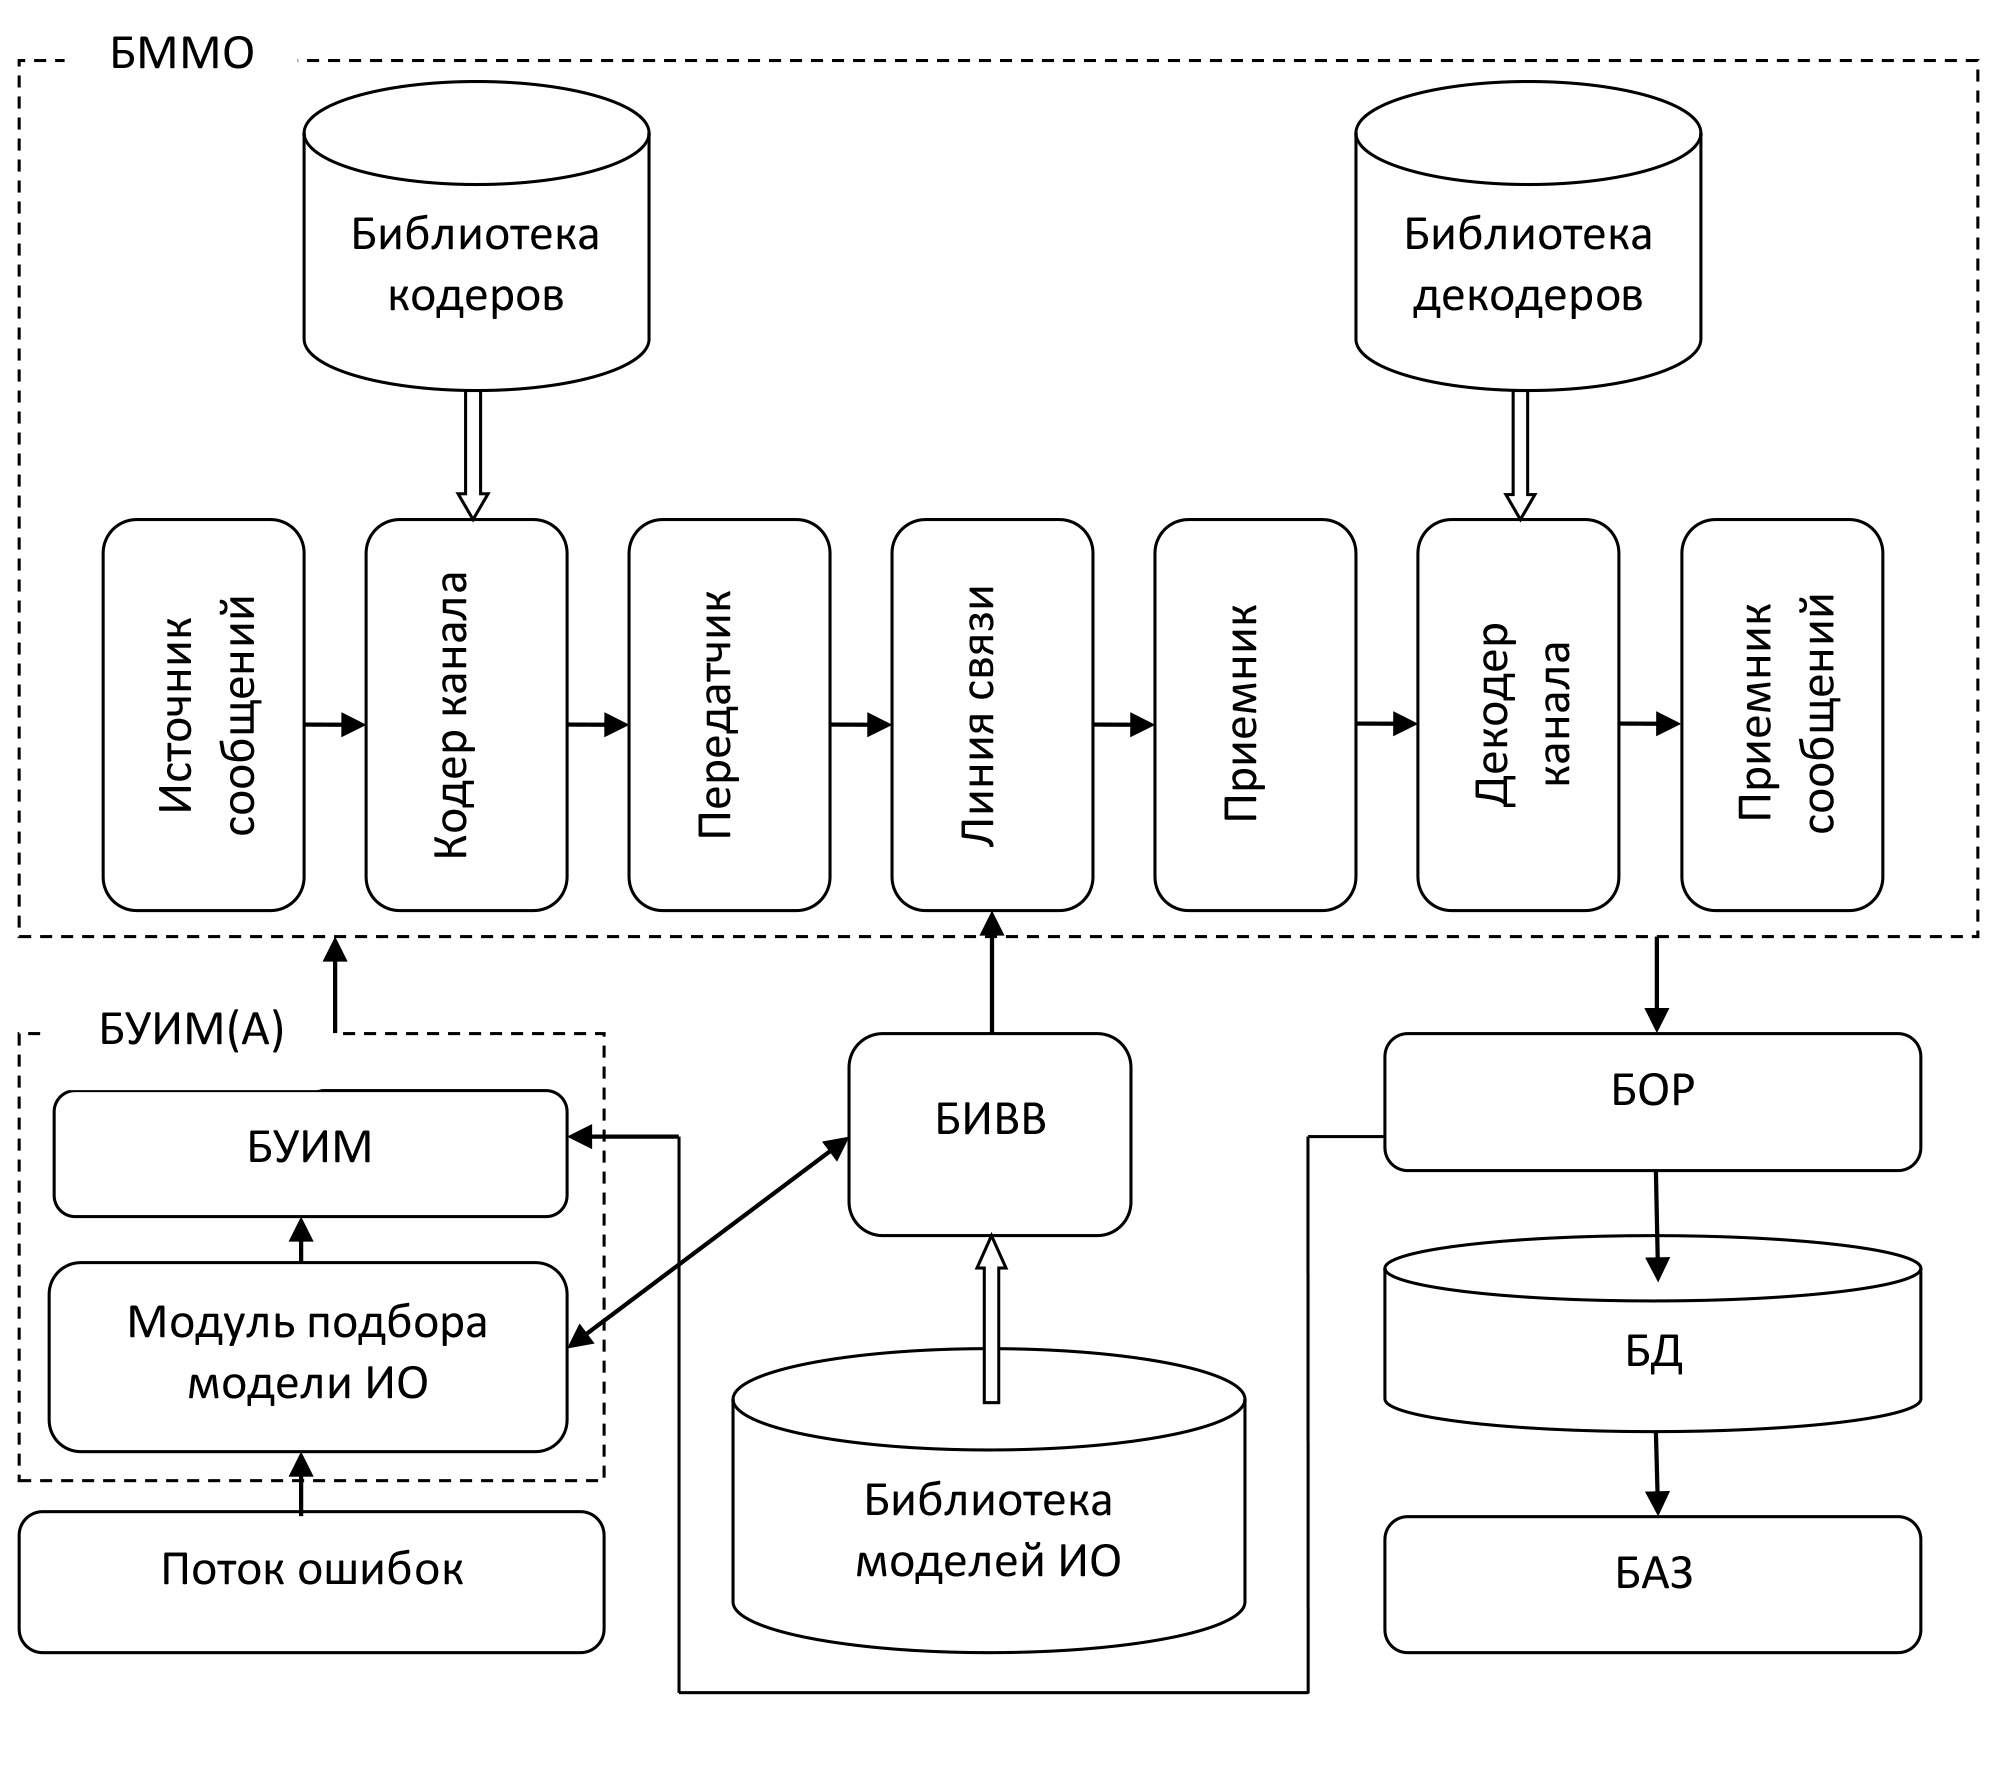
\includegraphics[height=100mm]{isopsapk_mod.jpg}

Рис.1 Модифицированная схема ИС ОПСАПК.
\end{center}

На вход БУИМ(А) подается последовательность наблюдений $O_{1:T}$. БУИМ передает эту последовательность МПМИО, который в соответствии с некоторым критерием $K$ определяет подмножество моделей источника ошибок $\Lambda_K=\{\lambda_i\}$ из БМИО, способных сгенерировать такую последовательность. Далее МПМИО с помощью метода подбора из предыдущего раздела выбирает из него наиболее адекватную модель $\lambda$.
Выбранная модель $\lambda$ возвращается в БУИМ, который запрашивает у БОР результаты $R_\lambda$ интересующих пользователя экспериментов, проведенных с участием этой модели. Если искомые результаты $R_\lambda$ найдены, то необходимость в проведении имитационных экспериментов отпадает. Если же эксперименты для выбранной модели еще не проводились, то модель $\lambda$ подается блоком управления на вход генератора потоков ошибок, который производит генерацию потока ошибок моделью $\lambda$, и БУИМ запускает имитационные эксперименты.

Далее в главе 4 описывается разработанный программный комплекс для моделирования и анализа потоков ошибок. Комплекс предоставляет пользователю удобный интерфейс ....

\vspace{-10mm} \begin{thebibliography}{99} \small
 \bibitem{BibZhd_2009}
\emph{Бибов А.Ю. , Жданова М. А.} Экспериментальное исследование аналога списочного декодера Сидельникова с использованием обобщенной марковской модели источника ошибок.
// Информационное противодействие угрозам  терроризма -- 2009. -- №~13. -- С.~151-153.

 \bibitem{BibZhd_2010}
\emph{Бибов А.Ю. , Жданова М. А.} Экспериментальное исследование аналога списочного декодера Сидельникова с использованием обобщенной марковской модели источника ошибок. // Материалы XI Международной научно-практической конференции «Информационная безопасность», часть 1, Таганрог: Изд-во ТТИ ЮФУ, 2010, с. 221-225.

\bibitem{DeZhda_Ivan}\emph{Деундяк В.М., Жданова М.А.} Обобщенная марковская модель источника ошибок q-ичного цифрового канала нескольких физических состояний. // Математика и ее приложения: ЖИМО. -- Иваново: ИвГУ. -- 2010. -- Выпуск 1 (7). --  С.34-40.

 \bibitem{DeZhda_Obozr10}\emph{Деундяк В.М., Жданова М.А.} О некотором обобщении  марковской математической модели источника ошибок. // Обозрение  прикладной и промышленной математики. -- 2010, т.17, №5, c.713-714.

 \bibitem{DeZhda_Obozr11}\emph{Деундяк В.М., Жданова М.А.} О применении скрытых марковских моделей в моделировании источников ошибок. // Обозрение  прикладной и промышленной математики. -- 2011. --Выпуск 3. --С. 488.

     \bibitem{DeZhda_Zap}\emph{Деундяк В.М., Жданова М.А.} Об аппроксимации потока ошибок в канале передачи данных на основе скрытых полумарковских QP-моделей // Тези доповідей VI Міжнародної науково-практичної конференції «Сучасні проблеми і досягнення в галузі радіотехніки, телекомунікацій та інформаційних технологій»,19-21 вересня 2012 р.,м. Запоріжжя,2012,С.109-110.

 \bibitem{DeZhda_VGU13}\emph{Деундяк В.М., Жданова М.А.} Полиномиальное представление скрытой полумарковской модели
фергюсоновского типа. // Вестник ВГУ, Серия: Системный анализ и информационные технологии -- 2013, №2, c.71-78.

\bibitem{DeZhd_DSTU14}\emph{Деундяк В.М., Жданова М.А.} Решение задачи оценивания  скрытых полумарковских QP-моделей. // Вестник ДГТУ, Т.14, № 4(79), 2014, с.5-16.

\bibitem{DeZhd_Toliatti}\emph{Жданова М.А.} Экспериментальное исследование решения задачи оценивания скрытой полумарковской QP-модели // Материалы всероссийской научно-практической школы-конференции по информационной безопасности «Вестник по безопасности», выпуск №7.-Тольятти, ВуиТ, 2014, с. 10-11.

\bibitem{DeZhda_Izvestia2015}\emph{Деундяк В.М., Жданова М.А.} О решении задачи оценивания скрытых полумарковских моделей фергюсоновского типа. // Известия вузов. Сев.-Кавк. Регион. Естественные науки. 2015. N 3,  с. 19-24.

\bibitem{DeMoZhd_Sim}\emph{Деундяк В.М., Жданова М.А., Могилевская Н.С.} Об автоматизированном выборе модели потока ошибок в информационной системе оценки применимости помехоустойчивого кодирования // Труды научной школы И.Б.Симоненко. Выпуск 2. Ростов-на-Дону: издательство ЮФУ, 2015.  с. 111-120.

\bibitem{Zhd_SFEDU15}\emph{Zhdanova M.A.} Inverse problems of HSMM-based mathematical modeling of jamming environment // Международная научная конференция «Современные методы и проблемы теории операторов и гармонического анализа и их приложения VI». Ростов-на-Дон, 26 апреля - 1 мая 2015г.  Материалы конференции. Изд. Центр ДГТУ, Ростов-на-Дону, 2015, с.185.

\bibitem{Zhd_China}\emph{Zhdanova M.A., Deundyak V.M.} Evaluation problem for general hidden semi-Markov error source model// Numerical algebra with applications. Procceding of 4 China-Russia conference. Rostov-on-Don: SFUP, 2015. P.156-159.

\bibitem{Zhd_Briks}\emph{Жданова М.А.} Об экспериментальном исследовании решения задачи оценивания некоторых скрытых полумарковских моделей. // Международной конференции молодых ученых стран БРИКС
«Сотрудничество стран БРИКС для устойчивого развития», Ростов-на-Дону, 24 – 26 сентября 2015г.  Материалы конференции.  с. XXX-XXX.

\bibitem{DeMoZhd_conf16}\emph{Деундяк В.М., Жданова М.А., Могилевская Н.С.} Автоматизированный выбор модели потока ошибок в информационной системе оценки применимости помехоустойчивого кодирования // Международная научная конференция «Современные методы и проблемы теории операторов и гармонического анализа и их приложения VI». Ростов-на-Дону, 24 – 29 апреля 2016г.  Материалы конференции. Изд. Центр ДГТУ, Ростов-на-Дону, 2016, с.157-158

\bibitem{DeMoZhd_DSTU}\emph{Деундяк В.М., Жданова М.А., Могилевская Н.С.} Решение задачи подбора модели источника ошибок в ИС ОПСАПК. // Вестник Донского государственного технического университета. 2017. №4(91), с. 107-115.

\end{thebibliography}

% Выходные данные типографии.
% Исправьте на требуемое!
% Количество листов ("Печ. л." и "Уч.-изд. л." должно быть не более 1.0
% для кандидатской и 2.0 для докторской!

\thispagestyle{empty}
\vfill
\footnotesize
\hrule
\medskip\noindent
Подписано к печати \_.\_.2009 \hskip 10mm
Заказ \hskip 28mm
Формат \ $60\times90/16$

\medskip\noindent
Печ.~л. \ 1.0 \hskip 16mm
Уч.-изд. л. \ 1.0 \hskip 16mm
Тираж \ 120 \hskip 16mm
Бесплатно
\medskip\hrule

\medskip\noindent
Отпечатано в \_

\medskip\noindent
%адрес организации
\_
\end{document}
